\documentclass[mathserif,9pt]{beamer}
\usepackage{multimedia}
%%\usepackage[utf8]{inputenc}
%%\usetheme{Warsaw}
%%\usetheme{Rochester}
%%\usecolortheme{whale}
\usepackage{hyperref}
\hypersetup{colorlinks=true,filecolor=red,pdfnewwindow=true,pdffitwindow=false}

\definecolor{oxygenorange}{HTML}{F7800A}
\definecolor{oxygengray}{HTML}{686868}
\definecolor{oxygenlightgray}{HTML}{EEEEEE}
\definecolor{oxygenblue}{HTML}{236EAF}
\definecolor{ox}{HTML}{111EAF}
\definecolor{my_purple}{HTML}{ca1885}
%%\definecolor{my_anis}{HTML}{b3ec51}
%%\definecolor{my_anis}{HTML}{c2ed3d}
\definecolor{my_anis}{HTML}{e3ed3d}
\definecolor{my_tilleul}{HTML}{9a9c16}
\definecolor{darkred}{HTML}{c21125}
\definecolor{my_green}{HTML}{88ac0c}

\definecolor{blue_bruz}{HTML}{235497}
\definecolor{b_bruz}{HTML}{207ede}
\definecolor{grey_bruz}{HTML}{50586d}
\definecolor{yellow_bruz}{HTML}{b7a170}

\setbeamercolor*{Title bar}{fg=white}


\def\H{{\mathcal H}}
\def\Hu{{\H^1}}
\def\Comp{{\;^{c}\,}}
\def\fint{{\int\hspace{-8mm}-}}

\def\a{{\alpha }}
\def\b{{\beta }}
\def\d{{\delta }}
\def\e{{\varepsilon}}
\def\o{{\omega}}
\def\ds{\displaystyle}

\def\ha{{\hat{a}}}
\def\hb{{\hat{b}}}
\def\hx{{\hat{x}}}
\def\vf{{\varphi}}
\def\Cau{{{\cal C}^{0,\alpha}(\Gamma_1)}}
\def\Cad{{{\cal C}^{0,\alpha}(\Gamma_2)}}
\def\R{\mathbf R}

%%%%%%%%%%%%%%%%%%%%%%%%%%%%%%%%%%%%%%%%%%%%%%%%%%%%%%%%%%%%%%%%%%%%%%%%%%%%%%%%%  


\begin{document}
\usebackgroundtemplate{}

%%--------------------------------------------------------------------------------
\begin{frame}

\textcolor{b_bruz}{\bf{\Large{My Presentation}}}
\vspace*{1cm}

\small{
Archit YADAV
\vspace*{10mm}

}
\end{frame}
%%--------------------------------------------------------------------------------
\begin{frame}
\small{

\textcolor{b_bruz}{\Large{\bf 1. Introduction - Who and Where?}}
\bigskip

I'm a master's student currently in \textcolor{blue}{M2 MoSIG} with specialization track as Human and Digital World Interaction (\textcolor{blue}{HDWI}).
\medskip

I come from India and I did my bachelor's from Shiv Nadar University (SNU), in Noida, a city within the Delhi NCR.
\bigskip

\textcolor{b_bruz}{\Medium{\bf 1.1 Why Grenoble?}}
\medskip

Grenoble being a very prominent research hub with variety of labs, a really nice place to for academic oriented students.
The nearby beautiful geography (mountains) made a plus point.

\begin{figure}[!tbp]
  \centering
  \begin{minipage}[b]{0.4\textwidth}
    \centering
    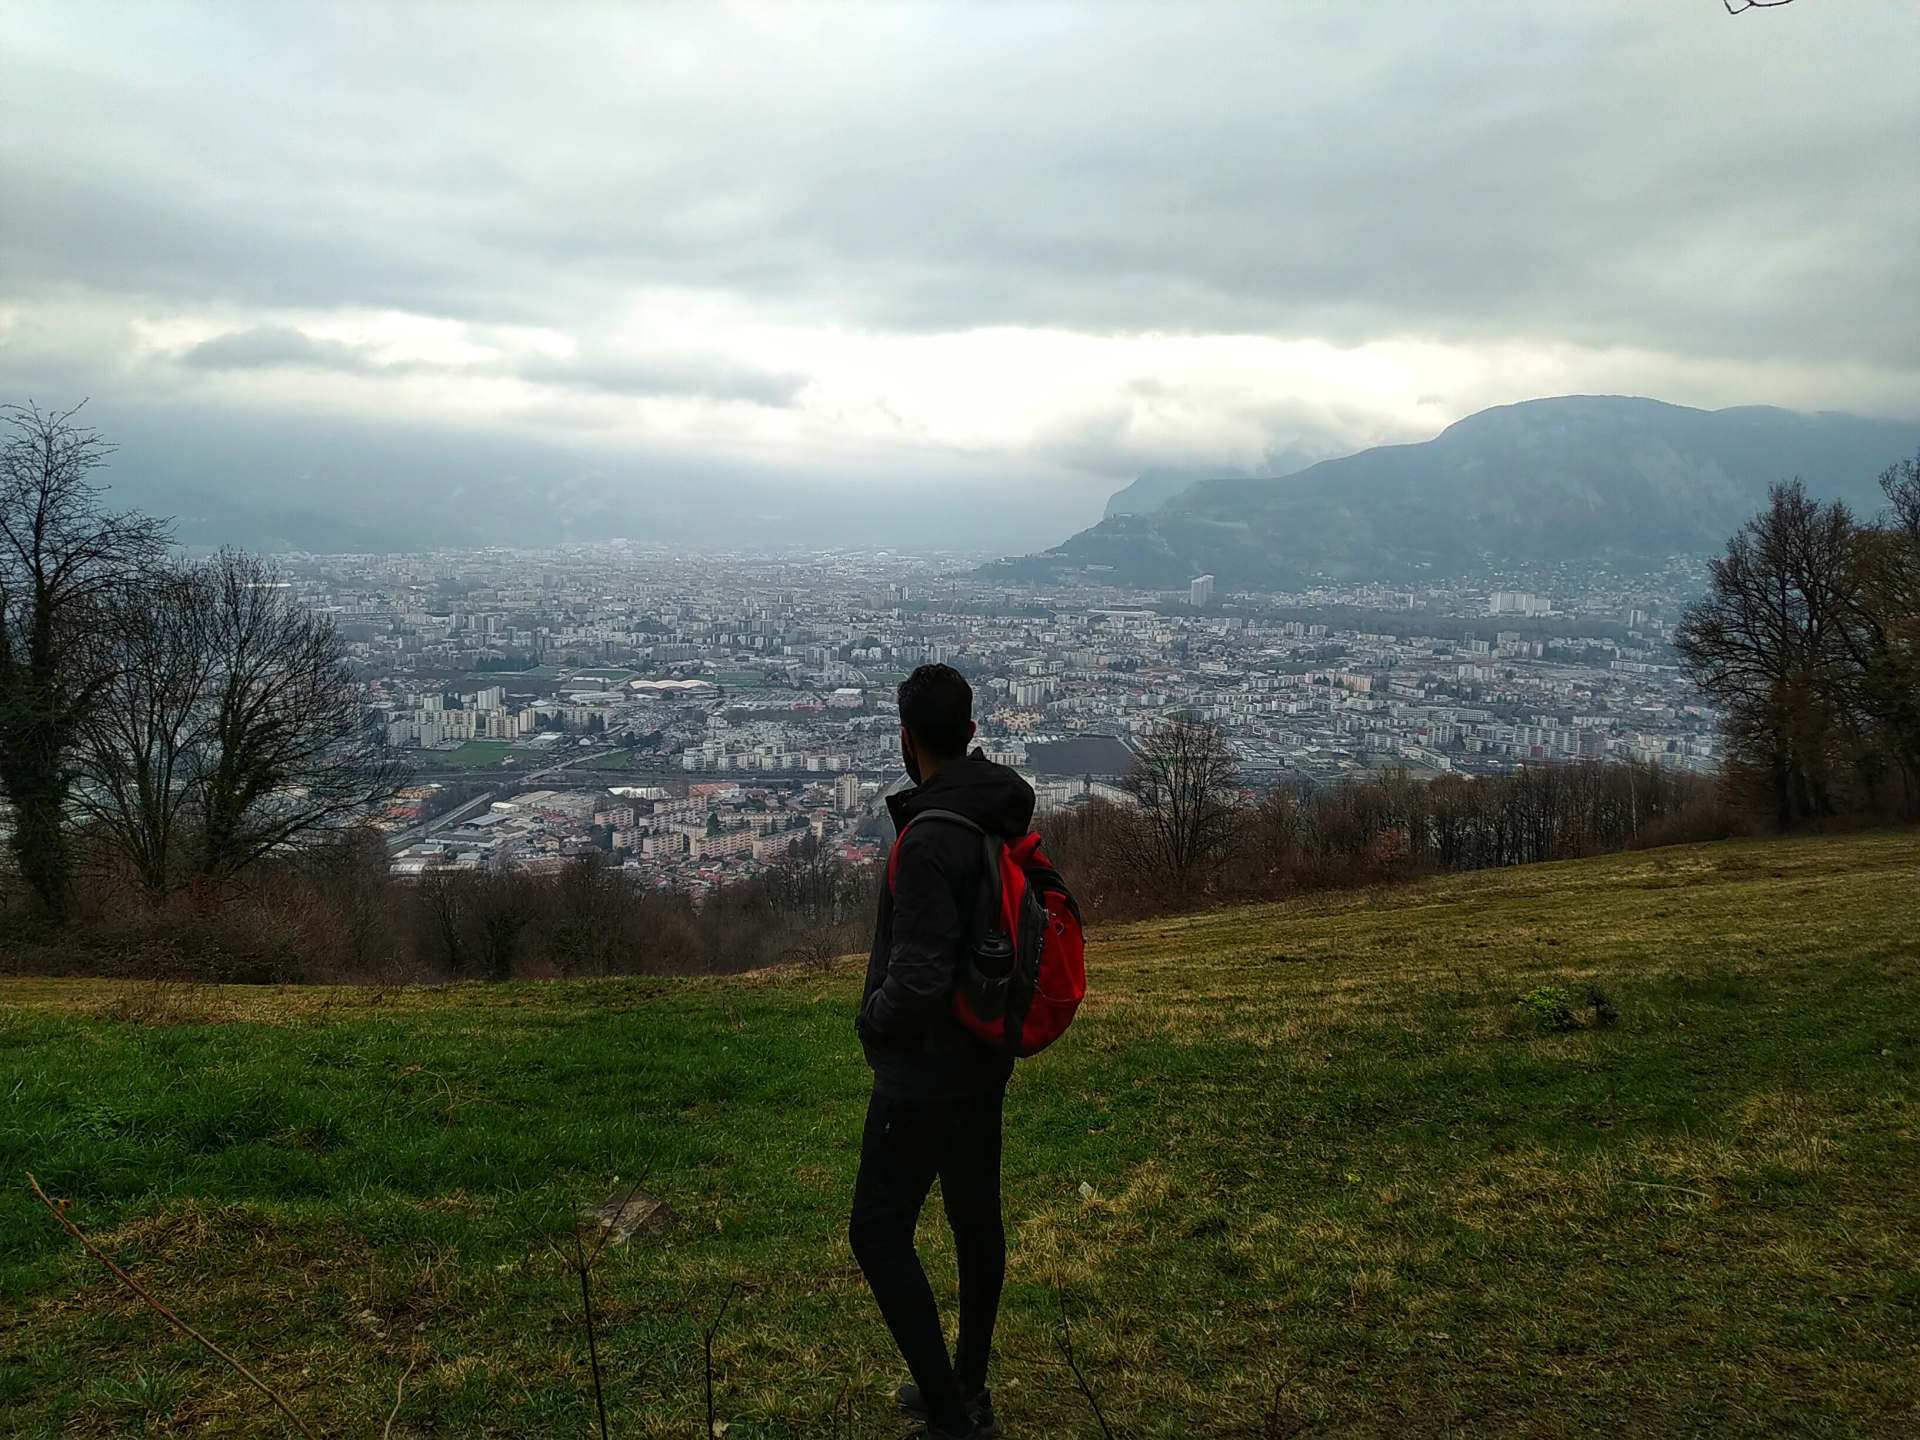
\includegraphics[height=3cm]{images/archit_hike_compressed.jpg}
  \end{minipage}
  \hfill
  \begin{minipage}[b]{0.4\textwidth}
    \centering
    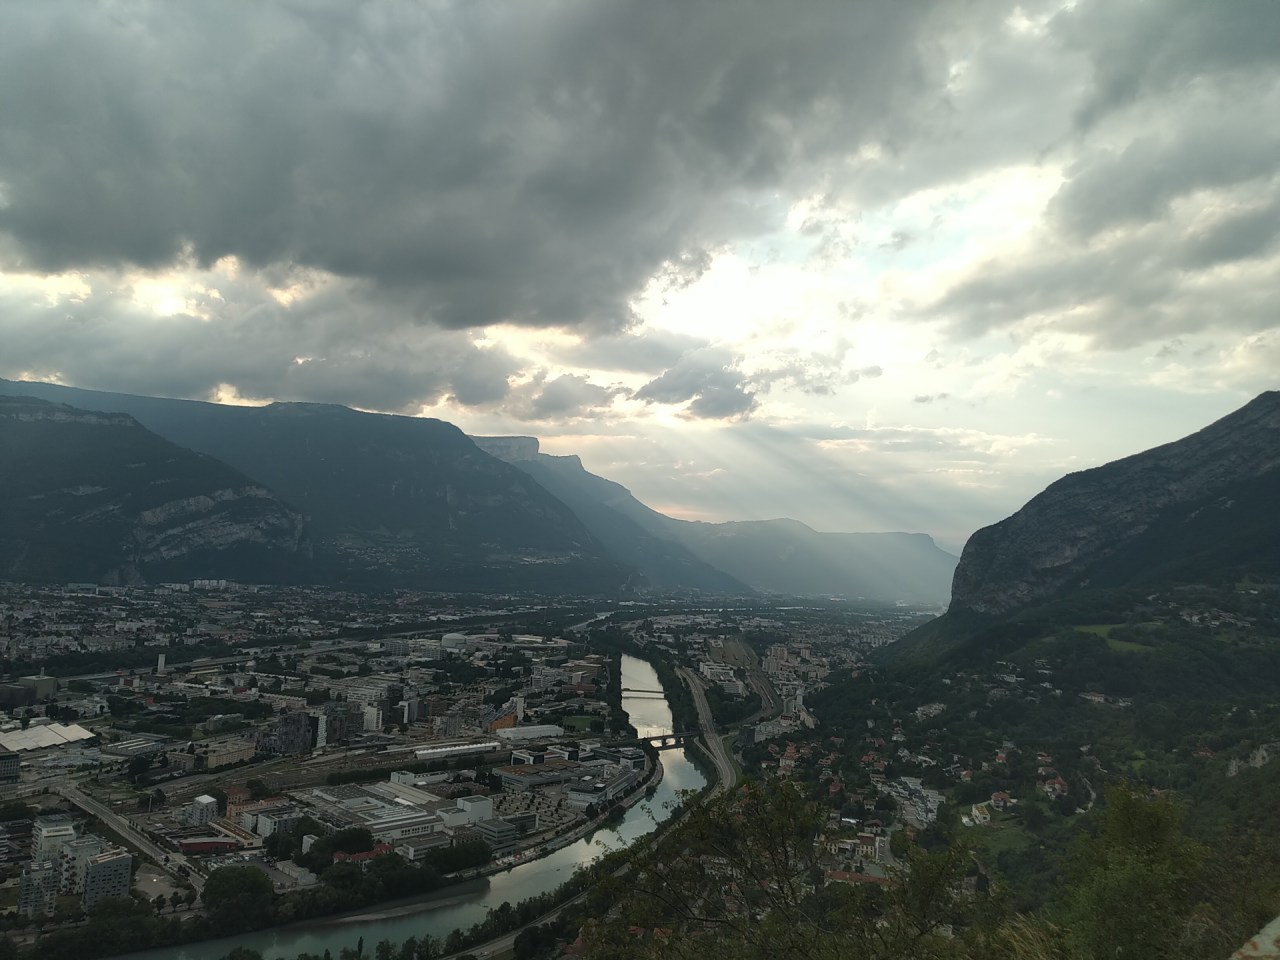
\includegraphics[height=3cm]{images/grenoble_bastille_top.jpg}
  \end{minipage}
\end{figure}


}
\end{frame}
%------------------------------------------------------------
\begin{frame}
\small{

\textcolor{b_bruz}{\Large{\bf 2. My Homeland - India}}

\begin{figure}[!tbp]
  \centering
  \begin{minipage}[b]{0.4\textwidth}
    \centering
    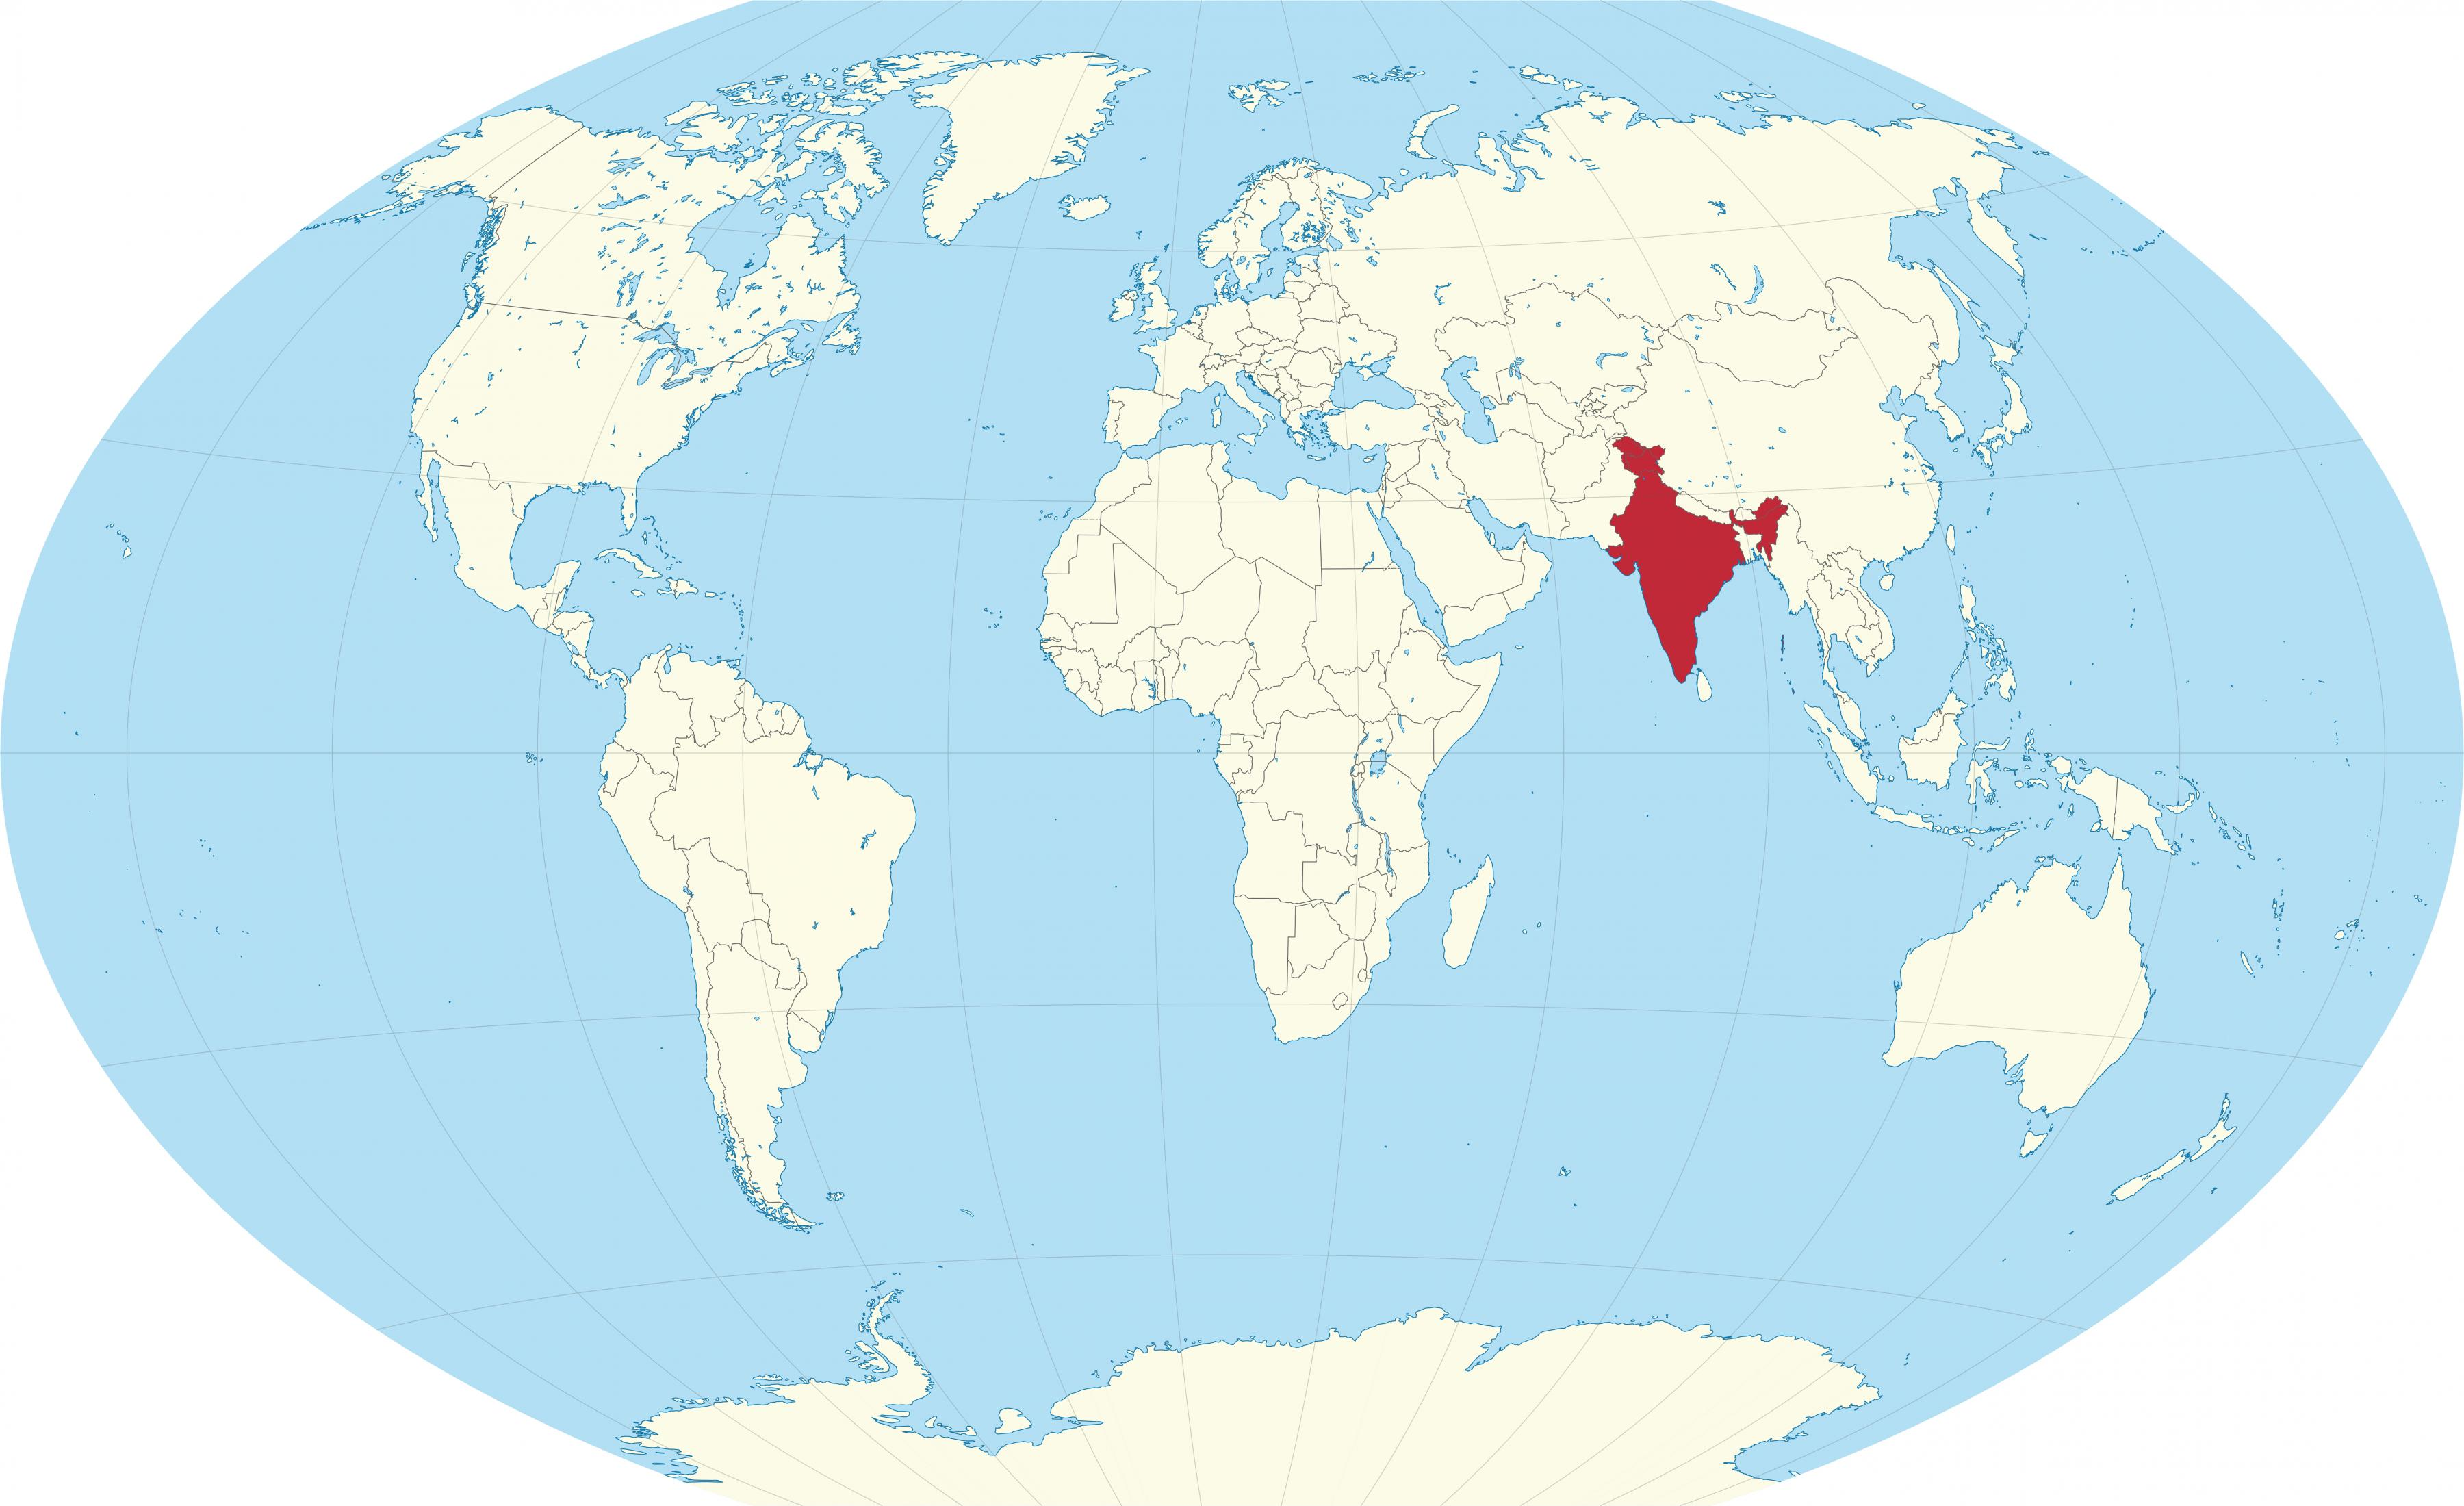
\includegraphics[height=3cm]{images/india-on-world-map.jpg}
  \end{minipage}
  \hfill
  \begin{minipage}[b]{0.4\textwidth}
    \centering
    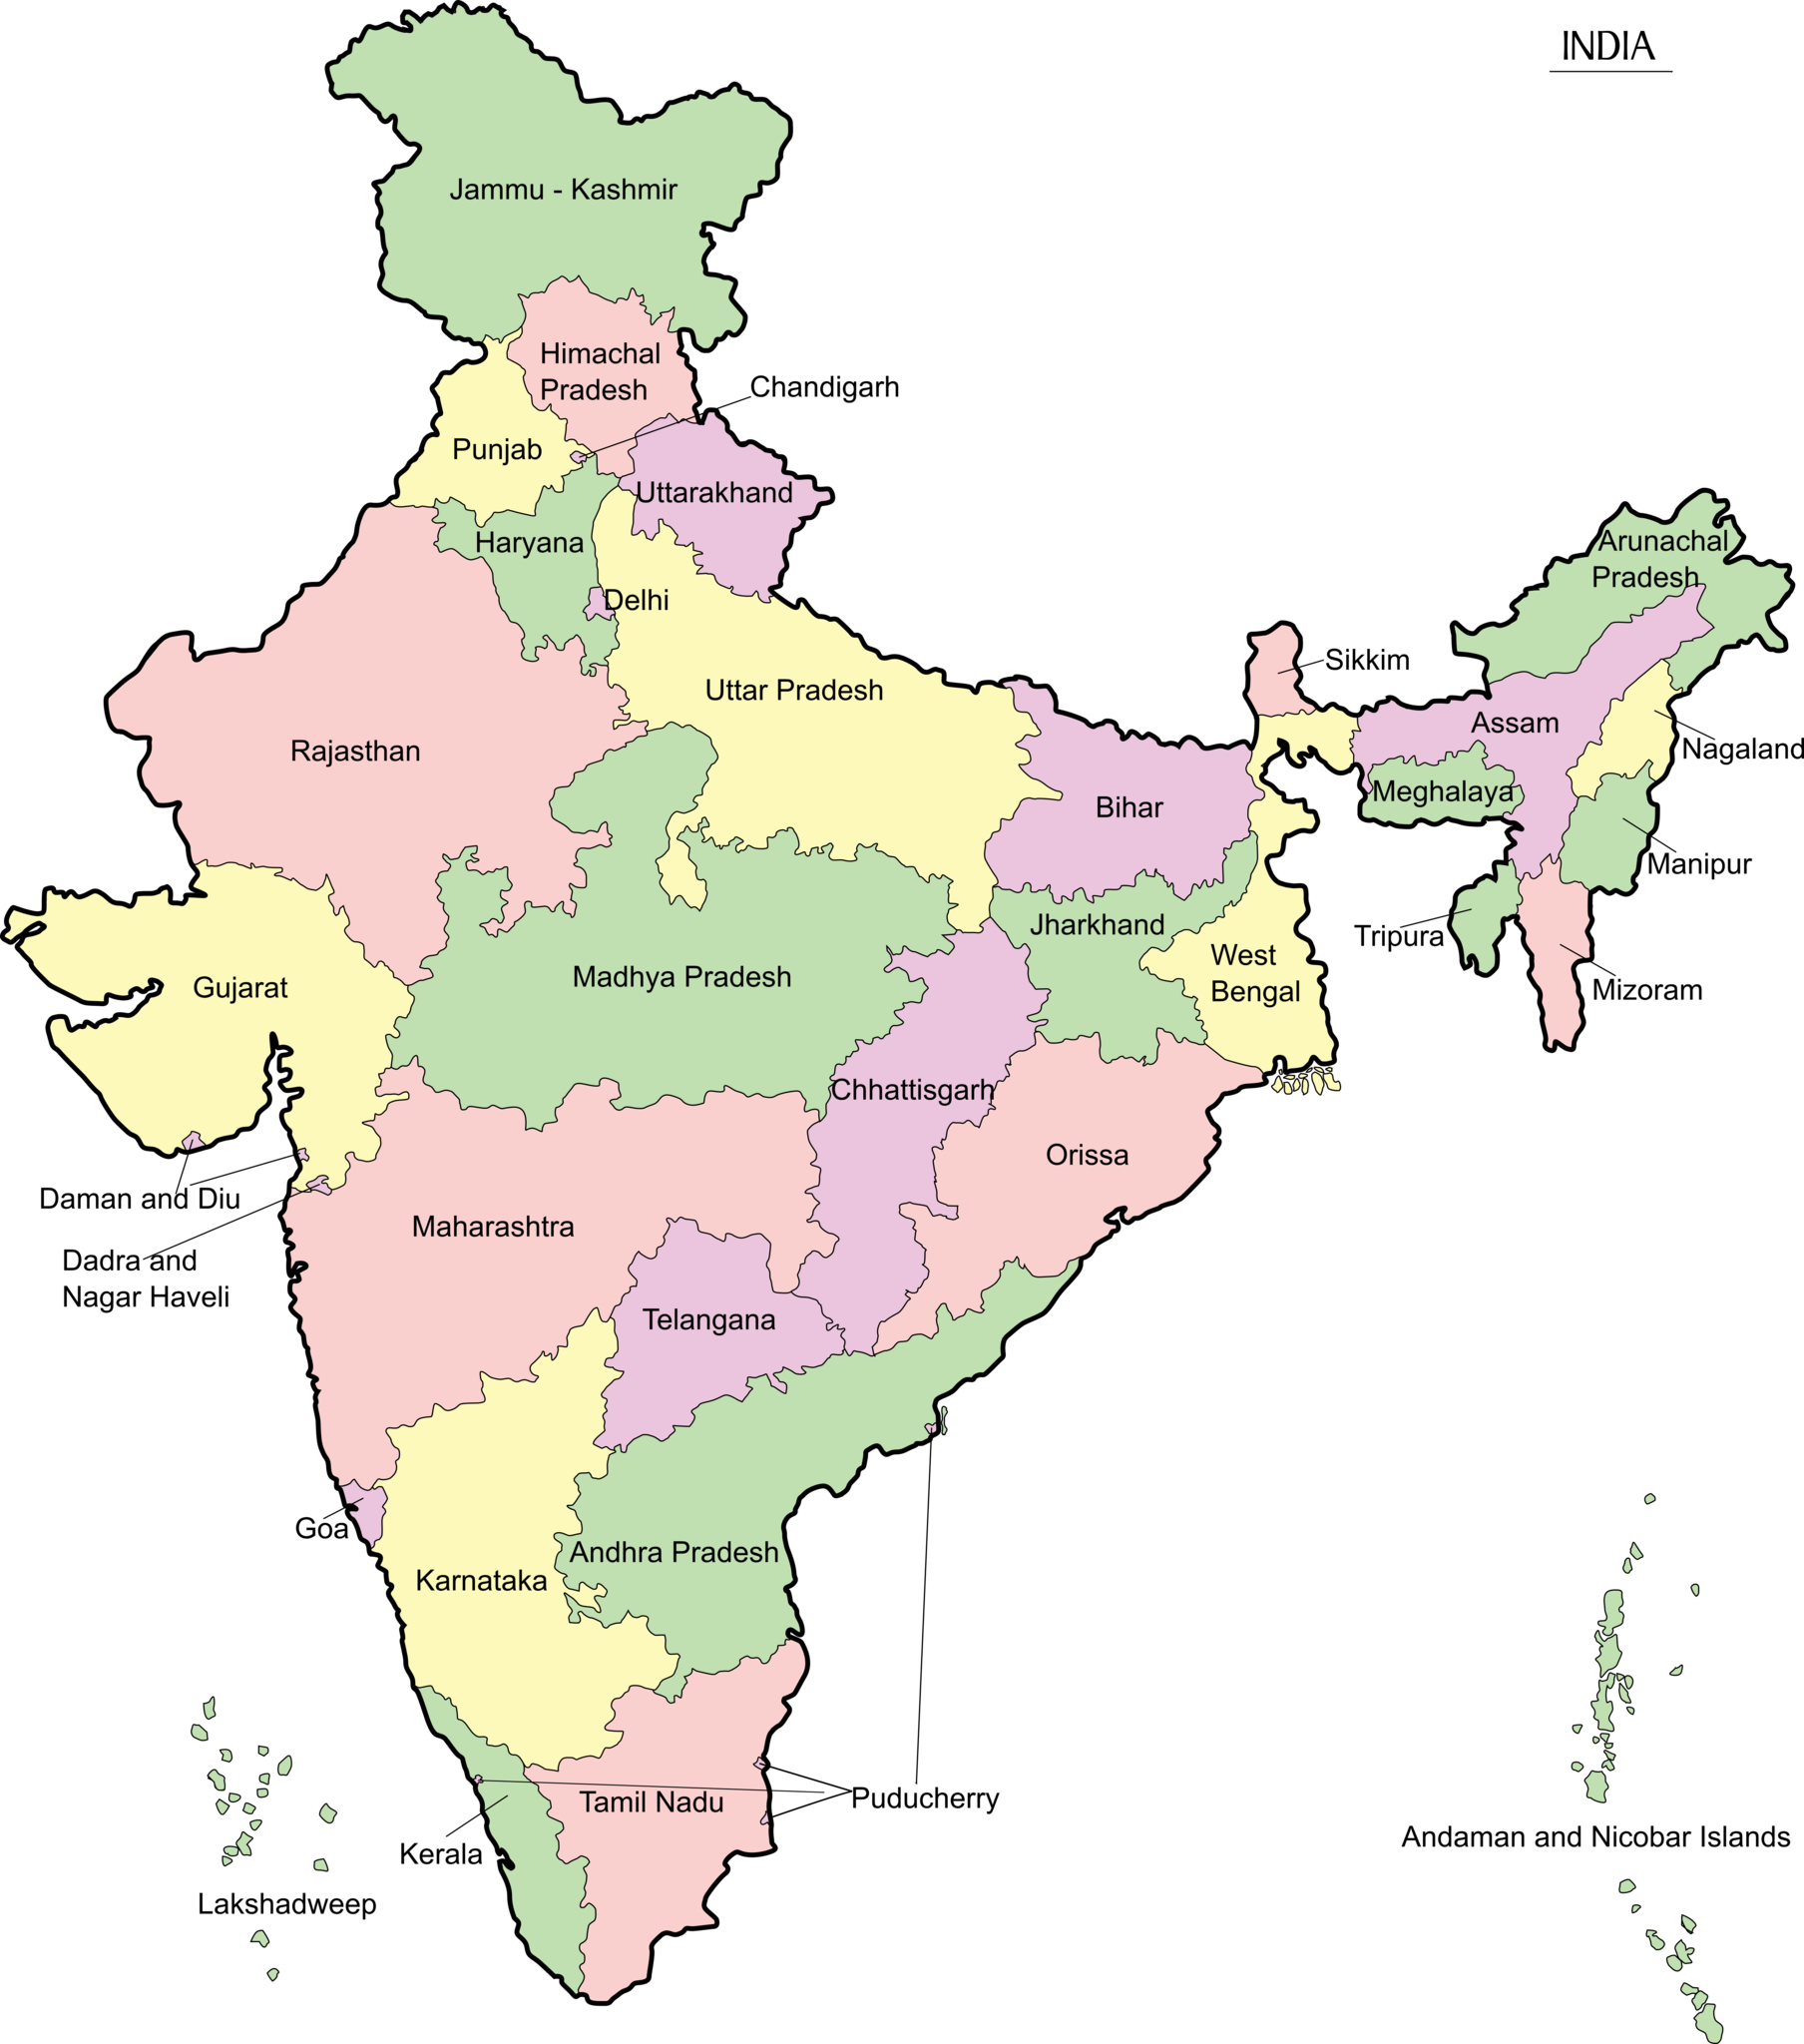
\includegraphics[width=3cm]{images/India-map-en.png}
  \end{minipage}
\end{figure}
\bigskip

\begin{itemize}
    \item[$\bullet$] Location - In South-Asia
    \item[$\bullet$] Capital - New Delhi
    \item[$\bullet$] College/University System
        \begin{itemize}
            \item Through nation/region-wide entrance exams
            \item CGPA (scale: 10) and percentage system
        \end{itemize}
    \item[$\bullet$] Some prominent scientists - 
        \begin{itemize}
            \item CV Raman (Scattering of light, Nobel Prize)
            \item APJ Abdul Kalam (\textit{"Missile Man of India"} and former president of India)
        \end{itemize}
    
\end{itemize}



}
\end{frame}
%------------------------------------------------------------
\begin{frame}
\small{

\textcolor{b_bruz}{\Large{\bf 3. My Website}}
\medskip

Checkout out my detailed information, some of my projects and other stuff on my personal website:
\smallskip

\href{https://archity.github.io}{archity.github.io} 
\bigskip

\textcolor{b_bruz}{\Medium{\bf Miscellanious}}
\medskip

One of my hobbies is \textcolor{blue}{drawing}, particularly digital art. Here are some of my works. More on my website. :D

\begin{figure}[!tbp]
  \centering
  \begin{minipage}[b]{0.4\textwidth}
    \centering
    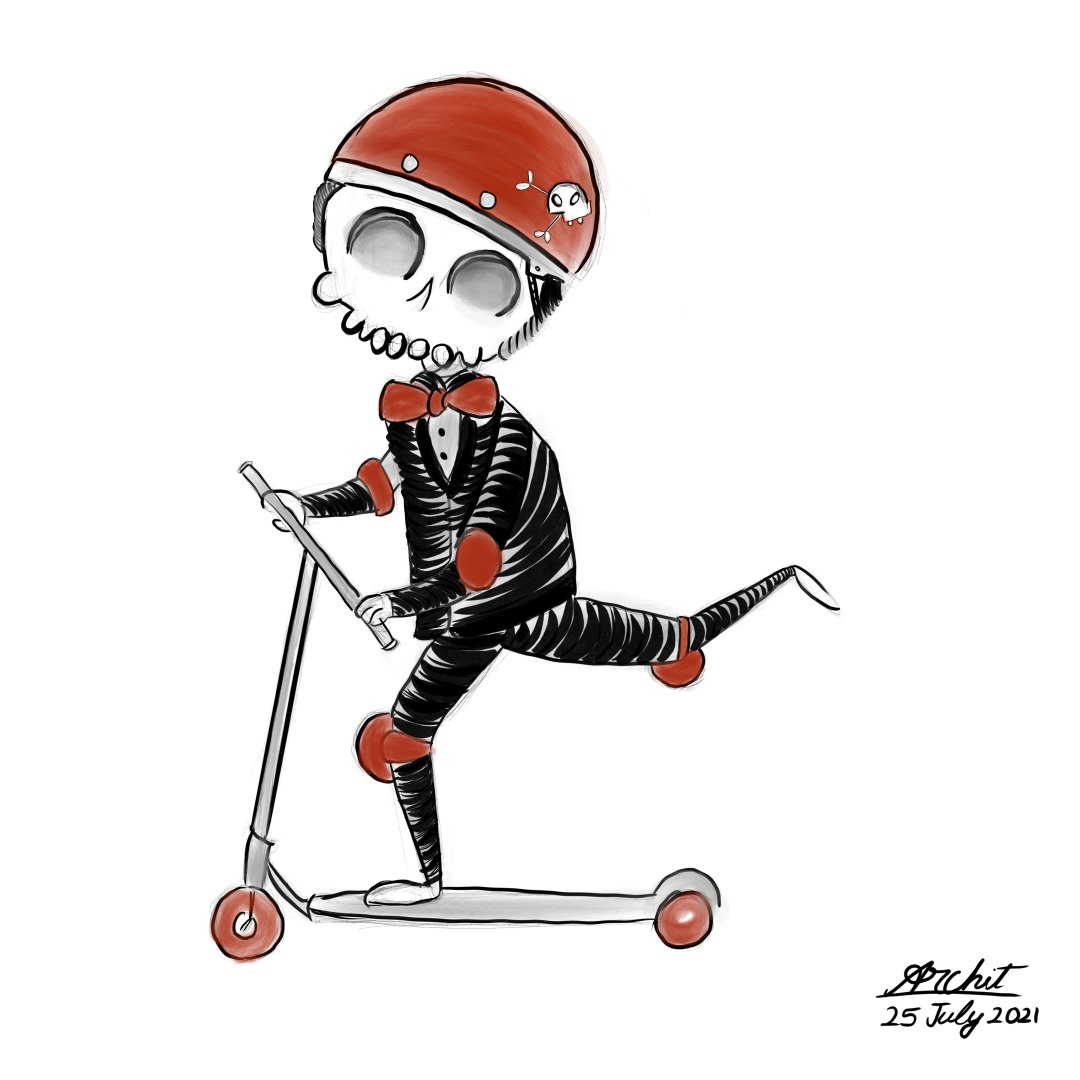
\includegraphics[width=3.5cm]{images/wally_procreate_compresed.jpg}
    \caption{Wally}
  \end{minipage}
  \hfill
  \begin{minipage}[b]{0.4\textwidth}
    \centering
    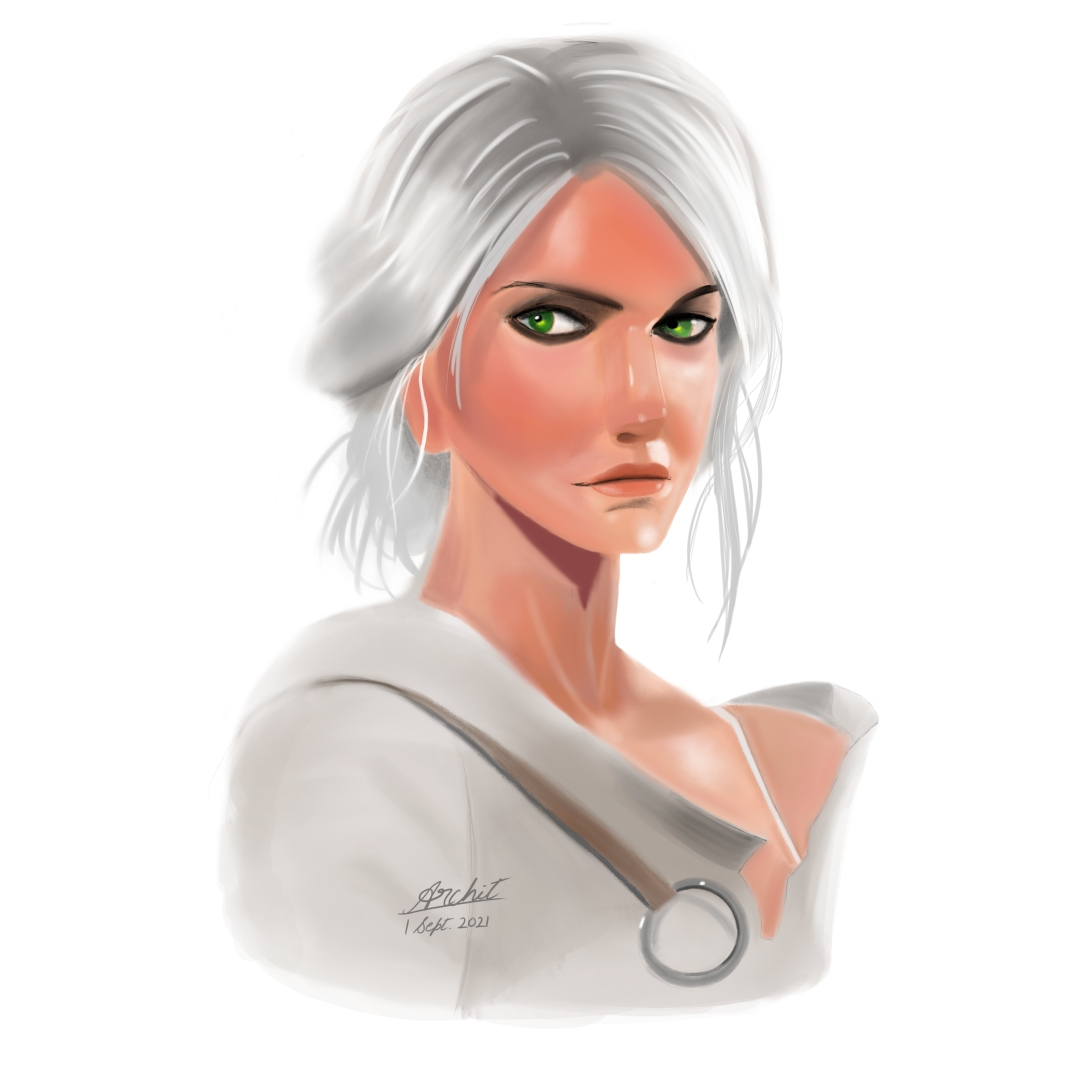
\includegraphics[width=3.5cm]{images/ciri_procreate_compressed.jpg}
    \caption{Ciri}
  \end{minipage}
\end{figure}



}
\end{frame}
%%--------------------------------------------------------------------------------


%%--------------------------------------------------------------------------------
\end{document}
%%--------------------------------------------------------------------------------





